% Use this template to write your solutions to COS 423 problem sets

\documentclass[12pt]{article}
\usepackage[utf8]{inputenc}
\usepackage{amsmath, amsfonts, amsthm, amssymb, algorithm, graphicx, mathtools, xfrac}
\usepackage[noend]{algpseudocode}
\usepackage{fancyhdr, lastpage}
\usepackage{booktabs}
\usepackage{multirow}
\usepackage{graphicx}
\usepackage{pgfplots}
\usepackage[vmargin=1.20in,hmargin=1.25in,centering,letterpaper]{geometry}
\setlength{\headsep}{.50in}
\setlength{\headheight}{15pt}

% Landau notation
\DeclareMathOperator{\BigOm}{\mathcal{O}}
\newcommand{\BigOh}[1]{\BigOm\left({#1}\right)}
\DeclareMathOperator{\BigTm}{\Theta}
\newcommand{\BigTheta}[1]{\BigTm\left({#1}\right)}
\DeclareMathOperator{\BigWm}{\Omega}
\newcommand{\BigOmega}[1]{\BigWm\left({#1}\right)}
\DeclareMathOperator{\LittleOm}{\mathrm{o}}
\newcommand{\LittleOh}[1]{\LittleOm\left({#1}\right)}
\DeclareMathOperator{\LittleWm}{\omega}
\newcommand{\LittleOmega}[1]{\LittleWm\left({#1}\right)}

% argmin and argmax
\newcommand{\argmin}{\operatornamewithlimits{argmin}}
\newcommand{\argmax}{\operatornamewithlimits{argmax}}

\newcommand{\calP}{\mathcal{P}}
\newcommand{\Z}{\mathbb{Z}}
\newcommand{\R}{\mathbb{R}}
\newcommand{\Exp}{\mathbb{E}}
\newcommand{\Q}{\mathbb{Q}}
\newcommand{\sign}{\mathrm{sign\ }}
\newcommand{\abs}{\mathrm{abs\ }}
\newcommand{\eps}{\varepsilon}
\newcommand{\zo}{\{0, 1\}}
\newcommand{\SAT}{\mathit{SAT}}
\renewcommand{\P}{\mathbf{P}}
\newcommand{\NP}{\mathbf{NP}}
\newcommand{\coNP}{\co{NP}}
\newcommand{\co}[1]{\mathbf{co#1}}
\renewcommand{\Pr}{\mathop{\mathrm{Pr}}}

% theorems, lemmas, invariants, etc.
\newtheorem{theorem}{Theorem}
\newtheorem{lemma}[theorem]{Lemma}
\newtheorem{invariant}[theorem]{Invariant}
\newtheorem{corollary}[theorem]{Corollary}
\newtheorem{definition}[theorem]{Definition}
\newtheorem{property}[theorem]{Property}
\newtheorem{proposition}[theorem]{Proposition}

% piecewise functions
\newenvironment{piecewise}{\left \{\begin{array}{l@{,\ }l}}
{\end{array}\right.}

% paired delimiters
\DeclarePairedDelimiter{\ceil}{\lceil}{\rceil}
\DeclarePairedDelimiter{\floor}{\lfloor}{\rfloor}
\DeclarePairedDelimiter{\len}{|}{|}
\DeclarePairedDelimiter{\set}{\{}{\}}

\makeatletter
\@addtoreset{equation}{section}
\makeatother
\renewcommand{\theequation}{\arabic{section}.\arabic{equation}}

% algorithms
\algnewcommand\algorithmicinput{\textbf{INPUT:}}
\algnewcommand\INPUT{\item[\algorithmicinput]}
\algnewcommand\algorithmicoutput{\textbf{OUTPUT:}}
\algnewcommand\OUTPUT{\item[\algorithmicoutput]}


% Formating Macros

\pagestyle{fancy}
\lhead{\sc \hmwkClass\ $\; \;\cdot \; \;$ \hmwkSemester\ $\; \;\cdot \; \;$
Problem \hmwkAssignmentNum.\hmwkProblemNum}
%\chead{\sc Problem \hmwkAssignmentNum.\hmwkProblemNum}
%\chead{}
\rhead{\em \hmwkAuthorName\ $($\hmwkAuthorID$)$\/}
\cfoot{}
\lfoot{}
\rfoot{\sc Page\ \thepage\ of\ \protect\pageref{LastPage}}
\renewcommand\headrulewidth{0.4pt}
\renewcommand\footrulewidth{0.4pt}

\fancypagestyle{fancycollab}
{
    \lfoot{\textit{Collaborators: \hmwkCollaborators}}
}

\fancypagestyle{problemstatement}
{
    \rhead{}
    \lfoot{}
}

%%%%%% Begin document with header and title %%%%%%%%%%%%%%%%%%%%%%%%%

\begin{document}

%%%%%% Header Information %%%%%%%%%%%%%%%%%%%%%%%%%%%%%%%%%%%%%%%%%%%

%%% Shouldn't need to change these
\newcommand{\hmwkClass}{COS 255}
\newcommand{\hmwkSemester}{Spring 2016}

%%% Your name, in standard First Last format
\newcommand{\hmwkAuthorName}{Lukas Leung}
%%% Your NetID
\newcommand{\hmwkAuthorID}{lleung}

%%% The problem set number (just the number)
\newcommand{\hmwkAssignmentNum}{6}

%%% The problem number (just the number)
\newcommand{\hmwkProblemNum}{1}

%%% A list of your collaborators' NetIDs, separated by ", ".
%%% You can use a new line ("\\") in the middle to prevent a long
%%% list from overflowing.
\newcommand{\hmwkCollaborators}{}
%%% Sets the collaborator list to appear on the first page
\thispagestyle{fancycollab}

%%%%%%% begin Solution %%%%%%%%%%%%%%%%%%%%%%%%%%%%%%%%%%%%%%%%%%%%
\section{Results from UVA}
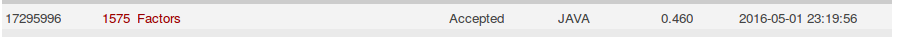
\includegraphics[width=\textwidth]{results}
% \newpage

%%%%%%% start Heavy Cargo %%%%%%%%%%%%%%%%%%%%%%%%%%%%%%%%%%%%%%%%%%

\section{UVA Problem 544: Heavy Cargo}
\textbf{Background} \\
~\indent  Big Johnsson Trucks Inc. is a company specialized in manufacturing big trucks.
Their latest model, the Godzilla V12 , is so big that the amount of cargo you can
transport with it is never limited by the truck itself. It is only limited by the weight
restrictions that apply for the roads along the path you want to drive. \\
\indent Given start and destination city, your job is to determine the maximum load of
the Godzilla V12 so that there still exists a path between the two specified cities. \\
\\
\textbf{Input} \\
\indent The input file will contain one or more test cases. The first line of each test case
will contain two integers: the number of cities $n\ (2 \leq n \leq 200)$ and the number of
road segments $r\ (1 \leq r \leq 19900)$ making up the street network. \\
\indent Then $r$ lines will follow, each one describing one road segment by naming the two
cities connected by the segment and giving the weight limit for trucks that use this
segment. Names are not longer than 30 characters and do not contain white-space
characters. Weight limits are integers $\in (0, 10000)$. Roads can always be travelled in
both directions. \\
\indent The last line of the test case contains two city names: start and destination. \\
\indent Input will be terminated by two values of 0 for $n$ and $r$. \\
\\
\textbf{Output} \\
\indent For each test case, print three lines:
\begin{itemize}
    \item a line saying "Scenario \#x" where $x$ is the number of the test case
    \item a line saying "y tons" where $y$ is the maximum possible load
    \item a blank line
\end{itemize}

%%%%%%% end Problem %%%%%%%%%%%%%%%%%%%%%%%%%%%%%%%%%%%%%%%%%%%%%%%

\newpage

%%%%%%% Mathematical Formulation %%%%%%%%%%%%%%%%%%%%%%%%%%%%%%%%%%
\subsection{Mathematical Formulation}
Given an input of $n$ cities, $c_1, c_2,..., c_n$, and $r$ roads with loads $l_1, l_2,..., l_r$ which connect
cities $c_i\ and\ c_j,\ 1 \leq i,j \leq r$, we will determine the maximum load that can be transported
from the specified cities ($a$ to $b$).

%%%%%%% Algorithm %%%%%%%%%%%%%%%%%%%%%%%%%%%%%%%%%%%%%%%%%%%%%%%%%

\subsection{Solution}
Important and potentially confusing data structures:
\begin{itemize}
    \item HashMap$\textless$String, Integer$\textgreater$ \textbf{cityIndex} : keeps track of the index associated
    with each city.
    \item int[n][n] \textbf{load} : ~ each element load[i][j] stores the highest constraining load that
    each road connecting city i and j.
    \item int[n] \textbf{curSet} : ~ stores the current row/column that we will add together for
    the Floyd-Warshall implementation.
    \item int[n][n] \textbf{l\_i} : ~ corresponding row/column sum that is calculated in each sub
    situation during the Floyd-Warshall algorithm.
\end{itemize}

The main functionality of this algorithm is an adapted Floyd-Warshall implementation
where we first build up our cityIndex HashMap and our load[ ][ ] which stores
the max load that each road can take between city "a" and city "b".

\begin{algorithm}[H]
\caption{Set-Up}
\begin{algorithmic}
    \Procedure{build}{Scanner in}
        \State $int senario \gets$ 0
        \While{true}
            \State $n, r \gets$ number of cities and number of roads from $in$
            \If{n == 0 and r == 0}
                break;
            \EndIf
            \State $load[n][n] and cityIndex \gets$ initialized
            \State $int lastIndex \gets$ 0
            \For{$i \in 0..(r-1)$}
                \State If not in hashmap put in.
                \State $int a, b \gets$ index of the two connected cities from $cityIndex$
                \State $int curLoad \gets$ the load specified by the file
                \State $load[a][b], load[b][a] \gets$ curLoad;
            \EndFor
            \State \Call{flyodWarshall}{load} // see Algorithm 2
            \State $int a, b \gets$ index of the two cities want to connect from $cityIndex$
            \State \Call{print}{load[a][b]}
        \EndWhile
    \EndProcedure
\end{algorithmic}
\end{algorithm}


The main difference comes from our rules, instead of using the rule:
\[ load(i, j, k) = \textbf{min}
\begin{cases}
    load(i, j, k-1) \\
    load(i, k, k-1) + load(k, j, k-1)
\end{cases}
\]
where i, j are the the correspoding cities i and j and i = j $\implies$ load(i,j,k) = 0 $\forall\ k$, we have
\[ load(i, j, k) = \textbf{max}
\begin{cases}
    load(i, j, k-1) \\
    load(i, k, k-1) + load(k, j, k-1)
\end{cases}
\]
One thing to note here is that we will be representing the distances seen so far in our
2-D array $load$ array. When implementing this the things to keep in mind are that
elements load[a][b] = load[b][a] always.

\begin{algorithm}[H]
\caption{Floyd-Warshall Implementation}
\begin{algorithmic}
    \Procedure{floydWarshall}{int[ ][ ] load}
        \State $curSet, l\_i \gets$ initialized
        \For{$i \in 0..(n-1)$}
            \For{$k \in 0..(n-1)$}
                \State $curSet[k] \gets$ load[i][k]
            \EndFor
            \State // build l\_i
            \For{$row \in 0..(n-1)$}
                \For{$col \in 0..(n-1)$}
                    \If{row == col}
                        continue;
                    \EndIf
                    \State $l\_i[row][col] \gets$ Math.\Call{min}{curSet[row], curSet[col]};
                \EndFor
            \EndFor
            \State // do dynamic step
            \For{$row \in 0..(n-1)$}
                \For{$col \in 0..(n-1)$}
                    \If{row == col}
                        continue;
                    \EndIf
                    \State $load[row][col] \gets$ Math.\Call{max}{load[row][col], l\_i[row][col]};
                \EndFor
            \EndFor
        \EndFor
    \EndProcedure
\end{algorithmic}
\end{algorithm}

%%%%%%% Correctness %%%%%%%%%%%%%%%%%%%%%%%%%%%%%%%%%%%%%%%%%%%%%%%

\subsection{Correctness}
%%%%%%% PROPOSITION 1 %%%%%%%%%%%%%%%
\begin{proposition}
~ \\ \indent Our adapted Floyd-Warshall Shortest Path Distance algorithm to a Floyd-Warshall
Highest Load algorithm sufficiently solves the problem.
\end{proposition}

\begin{proof}
~ \\ \indent In class we prooved that the Floyd-Warshall Shortest Path Distance algorithm
will determine the shortest path between two nodes given a "graph" with the edge
weights being the distance between two nodes. Now the dynamic algorithm rule that
we use to build this solution is expressed as:
\[ dist(i, j, k) = \textbf{min}
\begin{cases}
    dist(i, j, k-1) \\
    dist(i, k, k-1) + dist(k, j, k-1)
\end{cases}
\]
\[
where,\ dist(i, j, 0) =
\begin{cases}
    w_{i,j}\ if\ (i, j) \in E \\
    \infty\ if\ (i, j) \notin E \\
    0\ if\ i = j
\end{cases}
\]
Such that $w_{i,j}$ is the weight between nodes $i$ and $j$ and $E$ is the set of all edges. Now
we adapt this such that $E$ is all roads, $w_{i,j}$ is the load of each road between cities $i$
and $j$. Therefore we are no longer looking for distances, but loads $\implies dist \rightarrow load$
and instead of finding the min we are looking for the max. Therefore, we have the
new formulation:
\[ load(i, j, k) = \textbf{max}
\begin{cases}
    load(i, j, k-1) \\
    load(i, k, k-1) + load(k, j, k-1)
\end{cases}
\]
Which is the algorithm which we have implemented. Since this is the only difference with
the original, we can say that this is sufficient to solve the given problem.
\end{proof}


%%%%%%% Analysis %%%%%%%%%%%%%%%%%%%%%%%%%%%%%%%%%%%%%%%%%%%%%%%%%%
\subsection{Analysis}
For the following analysis, we will say that $N$ is the number of cities that are given
to us. We note here that all of the analysis is dependent on the number of cities and
not the number of roads. This is due to the fact that the roads are being represented
through our load[ ][ ] which is dependent on $N$ already.

%%%%%%% PROPOSITION 1 %%%%%%%%%%%%%%%
\begin{proposition}
\label{numq}
The \underline{space complexity} of this algorithm is \textbf{O(N$^2$)}
\end{proposition}

\begin{proof}
~ \\ \indent This is due to the fact that all of our data is stored in data structures:
\begin{itemize}
     \item HashMap$\textless$String, Integer$\textgreater$ \textbf{cityIndex} : stores indexes of all cities $\implies N$
    \item int[n][n] \textbf{load} : ~ stores the distances from cities a to b $\implies N^2$
    \item int[n] \textbf{curSet} : ~ stores the row/column distances that will be used to calculate l\_i $\implies N$
    \item int[n][n] \textbf{l\_i} : ~ stores the calculated distances from cities a to b ($N^2$) from  $curSet$ $\implies N^2$
    \item \underline{cause}: reason $\implies complexity$
\end{itemize}
At any point in time, there will exist at most one of each of these data structures $\implies$ $2\cdot N^2 + 2\cdot N$
\begin{center}
    $\therefore$ Giving us a space complexity of \textbf{O(N$^2$)}
\end{center}
\end{proof}

%%%%%%% PROPOSITION 2 %%%%%%%%%%%%%%%
\begin{proposition}
\label{numq}
The \underline{time complexity} of this algorithm is \textbf{O(N$^3$)}
\end{proposition}

\begin{proof}
This is the case because our algorithm is just the adjusted Floyd-Warshall
Algorithm which builds $N$, $N$x$N$ matricies. At each step, $n\ s.t.\ 1 \leq n \leq N$ we are
computing the $N$x$N$ matrix in linear time ($N^2$) and somparing each element to an
existing $N$x$N$ graph which is also done in linear time. Therefore we are going through
$N^2$ operations $N$ times.
\begin{center}
    $\therefore$ Giving us a time complexity of \textbf{O(N$^3$)}
\end{center}
\end{proof}

%%%%%%% Example %%%%%%%%%%%%%%%%%%%%%%%%%%%%%%%%%%%%%%%%%%%%%%%%%%%

\subsection{An Example}
Given the input: \\
4 3     \\
K S 100 \\
S U 80  \\
U M 120 \\
K M     \\
We build our initial matrix load[4][4]:
\[  load =
\begin{bmatrix}
    \textbf{0}   & \textbf{100} & \textbf{0}   & \textbf{0}   \\
    \textbf{100} & 0   & 80  & 0   \\
    \textbf{0}   & 80  & 0   & 120 \\
    \textbf{0}   & 0   & 120 & 0
\end{bmatrix}
\]
And we begin our Floyd-Warshall algorithm by computing l\_i with the rows bolded
above to produce (the altered load elements have been underlined):
\[  l\_1 =
\begin{bmatrix}
    0   & 0   & 0   & 0   \\
    0   & 0   & 0   & 0   \\
    0   & 0   & 0   & 0   \\
    0   & 0   & 0   & 0
\end{bmatrix}
\implies load =
\begin{bmatrix}
    0   & \textbf{100} & 0   & 0   \\
    \textbf{100} & \textbf{0}   & \textbf{80}  & \textbf{0}   \\
    0   & \textbf{80}  & 0   & 120 \\
    0   & \textbf{0}   & 120 & 0
\end{bmatrix}
\]
continuing computing l\_i with the rows bolded above to produce:
\[  l\_2 =
\begin{bmatrix}
    0   & 0   & 80   & 0   \\
    0   & 0   & 0   & 0   \\
    80   & 0   & 0   & 0   \\
    0   & 0   & 0   & 0
\end{bmatrix}
\implies load =
\begin{bmatrix}
    0   & 100 & \textbf{\underline{80}}  & 0   \\
    100 & 0   & \textbf{80}  & 0   \\
    \textbf{\underline{80}}  & \textbf{80}  & \textbf{0}   & \textbf{120} \\
    0   & 0   & \textbf{120} & 0
\end{bmatrix}
\]
continuing computing l\_i with the rows bolded above to produce:
\[  l\_3 =
\begin{bmatrix}
    0   & 80   & 0   & 80   \\
    80   & 0   & 0   & 80   \\
    0   & 0   & 0   & 0   \\
    80   & 80   & 0   & 0
\end{bmatrix}
\implies load =
\begin{bmatrix}
    0   & 100 & 80  & \textbf{\underline{80}}   \\
    100 & 0   & 80  & \textbf{\underline{80}}   \\
    80  & 80  & 0   & \textbf{120} \\
    \textbf{\underline{80}}  & \textbf{\underline{80}}  & \textbf{120} & \textbf{0}
\end{bmatrix}
\]
and computing the final l\_i with the rows bolded above to produce:
\[  l\_3 =
\begin{bmatrix}
    0   & 80   & 80   & 0   \\
    80   & 0   & 80   & 0   \\
    80   & 80   & 0   & 0   \\
    0   & 0   & 0   & 0
\end{bmatrix}
\implies load =
\begin{bmatrix}
    0   & 100 & 80  & 80   \\
    100 & 0   & 80  & 80   \\
    \textbf{80}  & 80  & 0   & 120 \\
    80  & 80  & 120 & 0
\end{bmatrix}
\]
Therefore since K correlates with index 0 and M with index 3, the maximum load is
then load[0][3] = 80 (as bolded above)


%%%%%%% end Heavy Cargo %%%%%%%%%%%%%%%%%%%%%%%%%%%%%%%%%%%%%%%%%%%


%%%%%%% end Solution %%%%%%%%%%%%%%%%%%%%%%%%%%%%%%%%%%%%%%%%%%%%%%

\end{document}